\section{Data-driven results}
In this section we present the results of the data-driven models.
We start by showing the numerical solution of the shallow water equations, then we present the predictions of the NN and FNO models.
Until now, we have mostly considered discountinuous initial conditions, but we will also consider smooth initial conditions in this section.
We solve the SWE with the following initial conditions:
\begin{equation}\label{eq:data-driven-initial-conditions-gauss}
    \begin{aligned}
        h(x, 0) &= h_0 \exp \left( \frac{-{(x-\mu)}^2}{2 \sigma^2} \right) ,\\
        u(x, 0) &= 0 , \\
    \end{aligned}
\end{equation}
where $h_0 = 1, \mu = 0.5, \sigma = 0.1$. 
The function $h(x, 0)$ is a Gaussian function, illustrated in Figure~\ref{fig:NN_initial_1D}.
\begin{figure}[H]
    \centering
    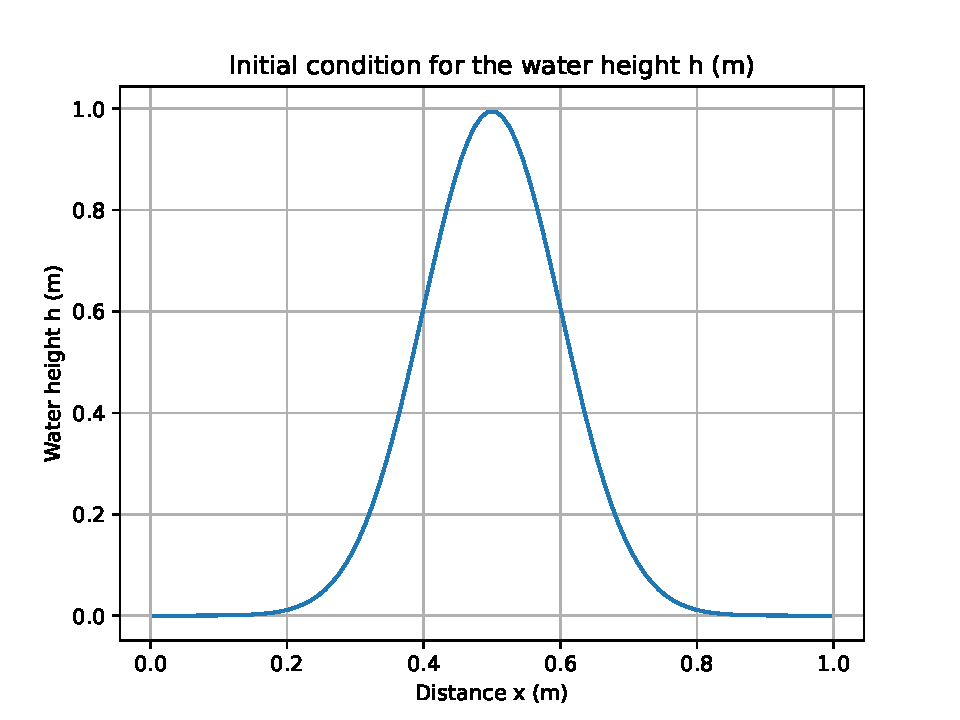
\includegraphics[width=0.5\textwidth]{C:/Users/Matteo/Shallow-Water-Equations/plots/NN_initial_1D.pdf}
    \caption{Initial conditions~\eqref{eq:data-driven-initial-conditions-gauss}.} \label{fig:NN_initial_1D}
\end{figure}
The domain is $ x \in [0, 1]$ with $N = 200$ points and the final time is $t = 1.0$.
We use a CFL number of $0.9$ and variable time steps.
The numerical solution is shown in Figure~\ref{fig:NN_initial}, in both a contour plot and a 3D plot.
\begin{figure}[H]
    \centering
    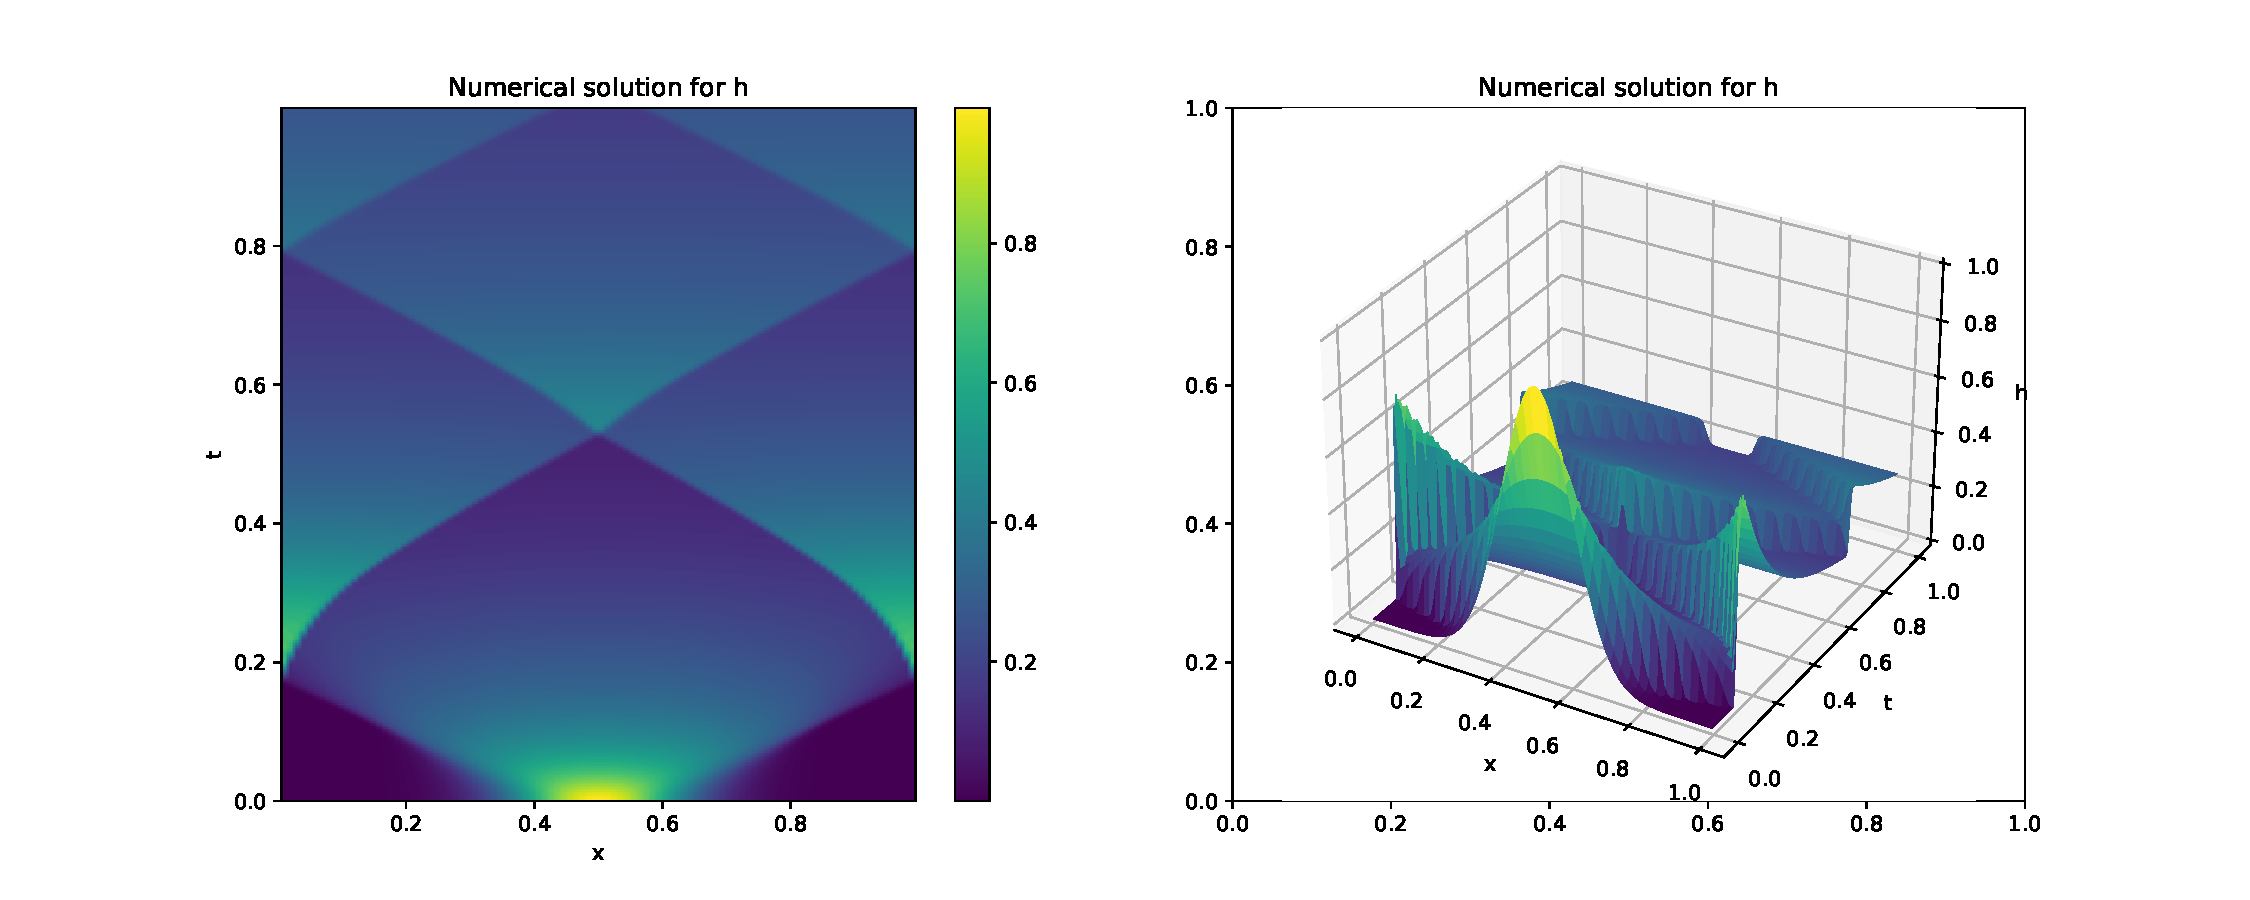
\includegraphics[width=0.7\textwidth]{C:/Users/Matteo/Shallow-Water-Equations/plots/NN_initial.pdf}
    \caption{Numerical solution of the shallow water equations with initial conditions~\eqref{eq:data-driven-initial-conditions-gauss}.}\label{fig:NN_initial}
\end{figure}


\subsection{RNN}
In the recurrent neural network, we train the model using the data generated by the numerical solution of the shallow water equations.
The model uses the data from the numerical solution to predict the solution at the next time step.
Meaning that the input and output data are the same, but shifted one time step.
This way, the model is supposed to learn the flowmap.
The RNN model consists of 4 layers.
%The neural network consists of the following layers: a input dense layer, three hidden dense layers with ReLU activation functions, a batch normalization layer for stability, a dropout layer to prevent overfitting, and an output dense layer.
The model has been trained using the Adam optimizer with a learning rate of $0.001$, a batch size of $32$ and a total of $500$ epochs.
We train the model on the data from $t = 0$ to $t = 0.8$, and test it on the data from $t = 0.8$ to $t = 1.0$.
The predictions of the model are shown in \autoref{fig:NN_predictions}.
\begin{figure}[H]
    \centering
    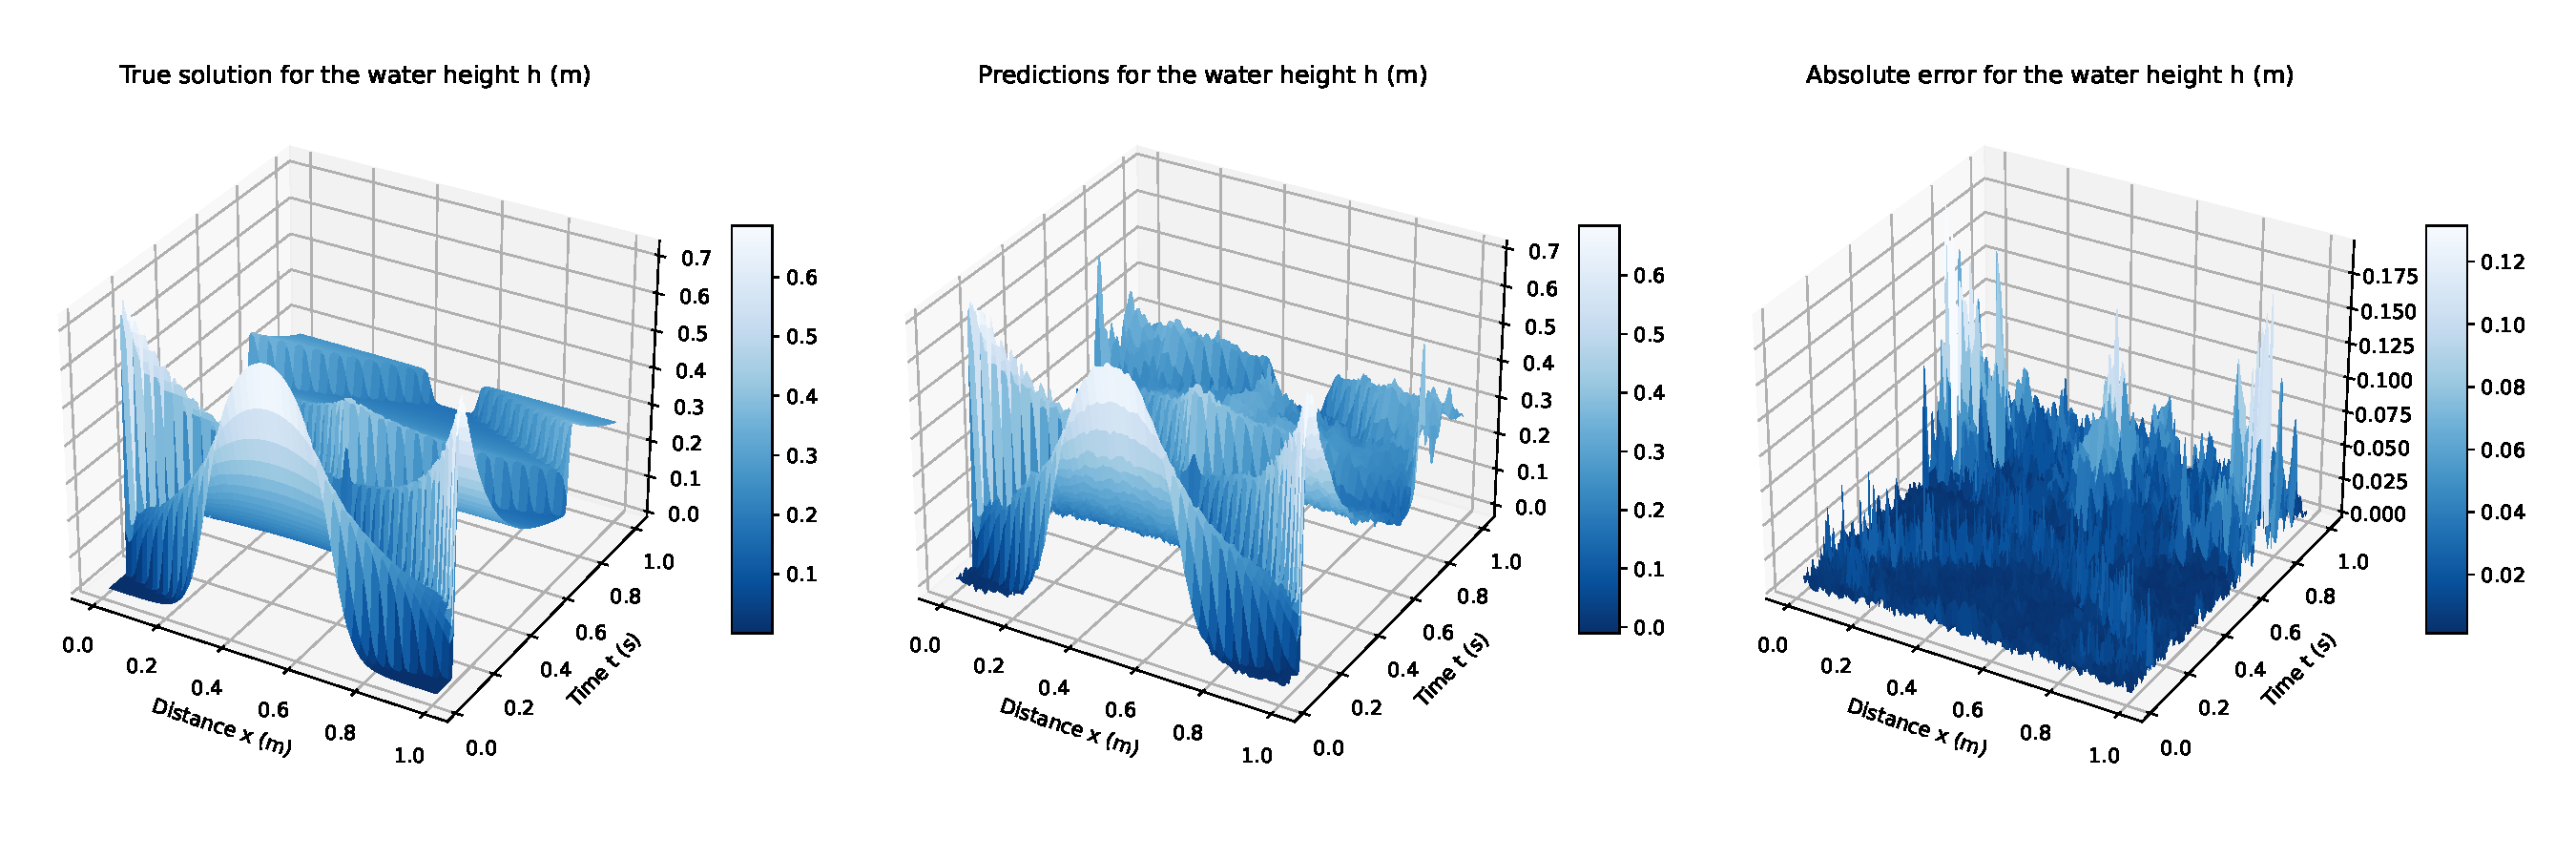
\includegraphics[width=0.99\textwidth]{C:/Users/Matteo/Shallow-Water-Equations/plots/NN_predictions.pdf}
    \caption{Predictions.}\label{fig:NN_predictions}
\end{figure}
From \autoref{fig:NN_predictions} we see that the neural network, is able to learn the dynamics of the solution, but the predictions are not accurate enough.
We also see that the highest absolute errors are located at the edges of the solution, which is expected, as the solution tends to be discontinuous.
We also see that the further we get in time, the worse the predictions become. This is also somehow expected, since we are outside the training data.
The training and validation loss is shown in \autoref{fig:NN_loss_train_val}.
\begin{figure}[H]
    \centering
    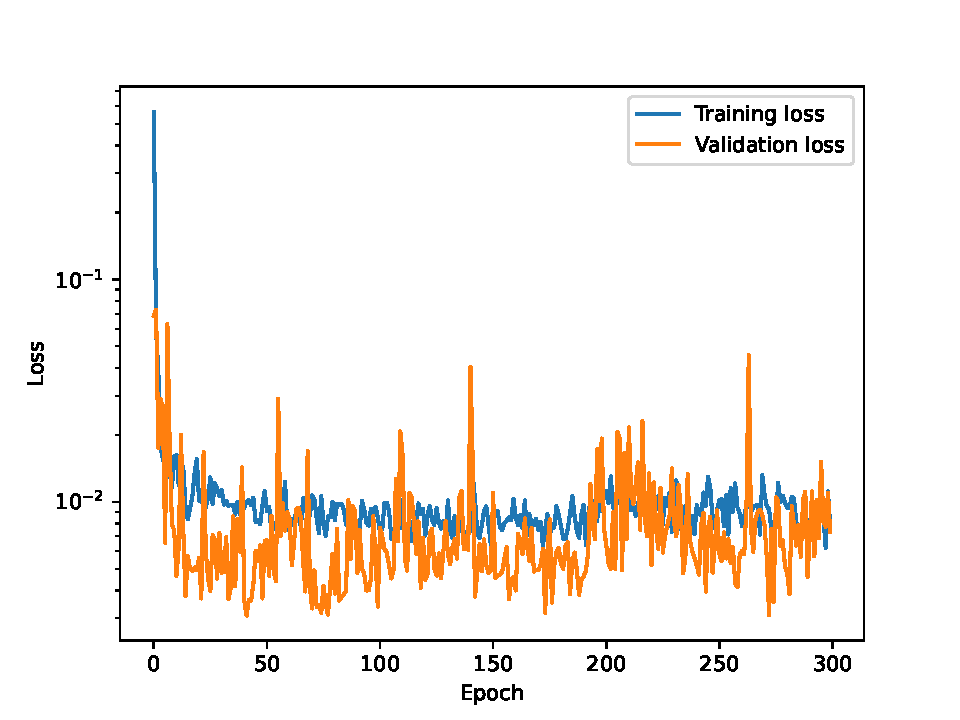
\includegraphics[width=0.6\textwidth]{C:/Users/Matteo/Shallow-Water-Equations/plots/NN_loss_train_val.pdf}
    \caption{Training and validation loss.}\label{fig:NN_loss_train_val}
\end{figure}
From \autoref{fig:NN_loss_train_val}, we see that a higher number of epochs, would probably not be beneficial, as the validation loss is increasing after a certain number of epochs.
Based on the training and validation loss, the model is overfitting the data. We see that as the training loss is decreasing, the validation loss is increasing.
This also means that the model is not able to generalize the data.
A possible solution could be to use more data.
To understand the performance of the model, we consider the predictions for some given time steps, shown in \autoref{fig:NN_predictions_time_steps}.
\begin{figure}[H]
    \centering
    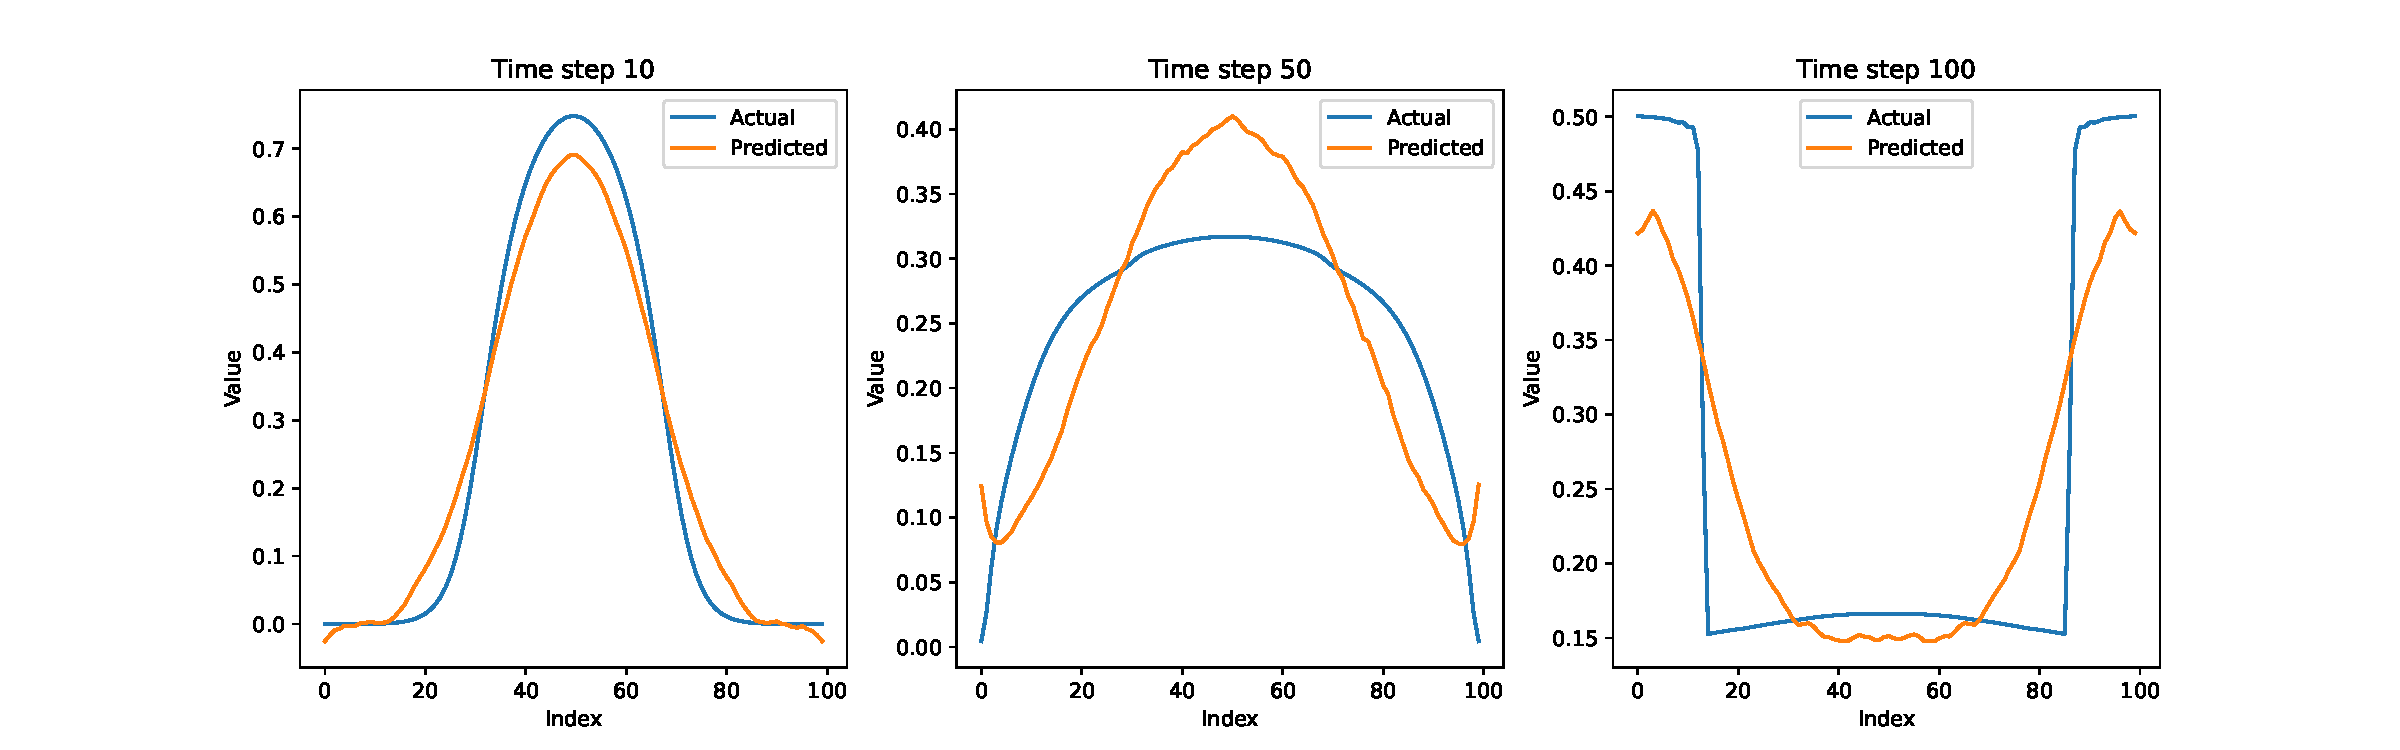
\includegraphics[width=0.95\textwidth]{C:/Users/Matteo/Shallow-Water-Equations/plots/NN_predictions_time_steps.pdf}
    \caption{Predictions for some given time steps.}\label{fig:NN_predictions_time_steps}
\end{figure}
Again, we see that the model finds some of the dynamics, but has many oscillations.
We have also trained a FNN model and a LSTM model, but the results are not shown here, as the performance is worse than the RNN model.


\subsection{FNO}
One of the main goals in this thesis is to use Fourier Neural Operators to solve the shallow water equations.
We define a FNO model, which consists of an input channel, 64 hidden channels and an output channel. We use a Fourier basis with 16 modes and a batch size of 32.
The model is trained using the Adam optimizer with a learning rate of $0.001$, a total of $1000$ epochs and the critera is to minimize the mean squared error (MSE).
The model is trained on the same data as the RNN model, and tested on the same data.
The results of the model are shown in \autoref{fig:FNO_predictions}.
\begin{figure}[H]
    \centering
    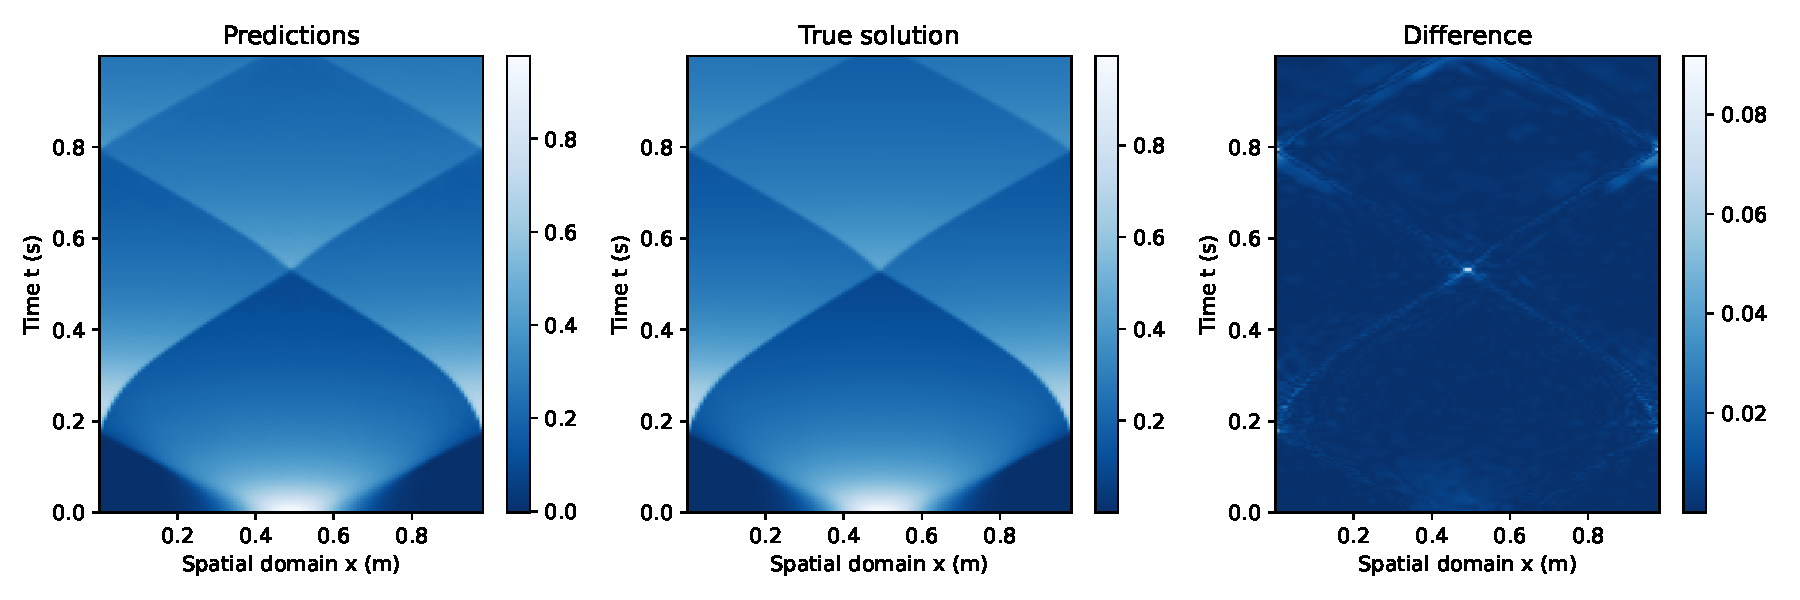
\includegraphics[width=0.9\textwidth]{C:/Users/Matteo/Shallow-Water-Equations/plots/pred_swe_epochs1000_channels64_lr_0.001.pdf}
    \caption{FNO predictions.}\label{fig:FNO_predictions}
\end{figure}
From \autoref{fig:FNO_predictions} we see that the FNO model is able to learn the dynamics of the solution, and it is able to predict the solution with high accuracy.
From the figure we also see that the error follows the edges of the solution, which is expected, as the solution tends to be discontinuous.
The loss for each iteration, which is epochs $\times$ batches, is shown in \autoref{fig:FNO_loss}.
\begin{figure}[H]
    \centering
    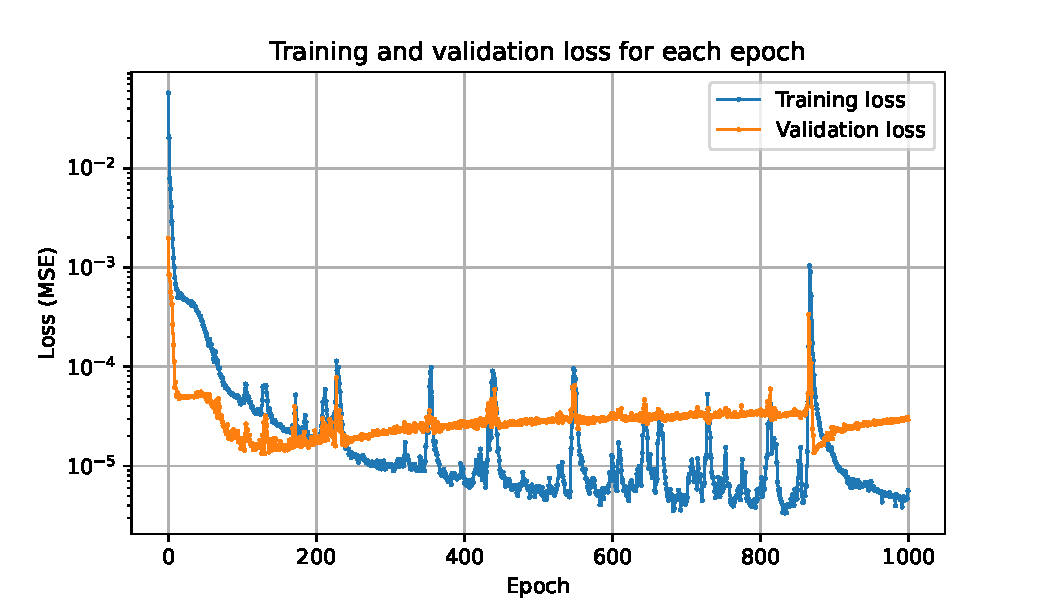
\includegraphics[width=0.7\textwidth]{C:/Users/Matteo/Shallow-Water-Equations/plots/loss_swe_epochs1000_channels64_lr_0.001.pdf}
    \caption{FNO loss.}\label{fig:FNO_loss}
\end{figure}
From \autoref{fig:FNO_loss} we see that the loss is decreasing for each iteration, and the model is able to learn the dynamics of the solution.
To get a deeper understanding of the performance of the model, we consider the predictions for some given time steps, shown in \autoref{fig:FNO_predictions_time_steps}.
\begin{figure}[H]
    \centering
    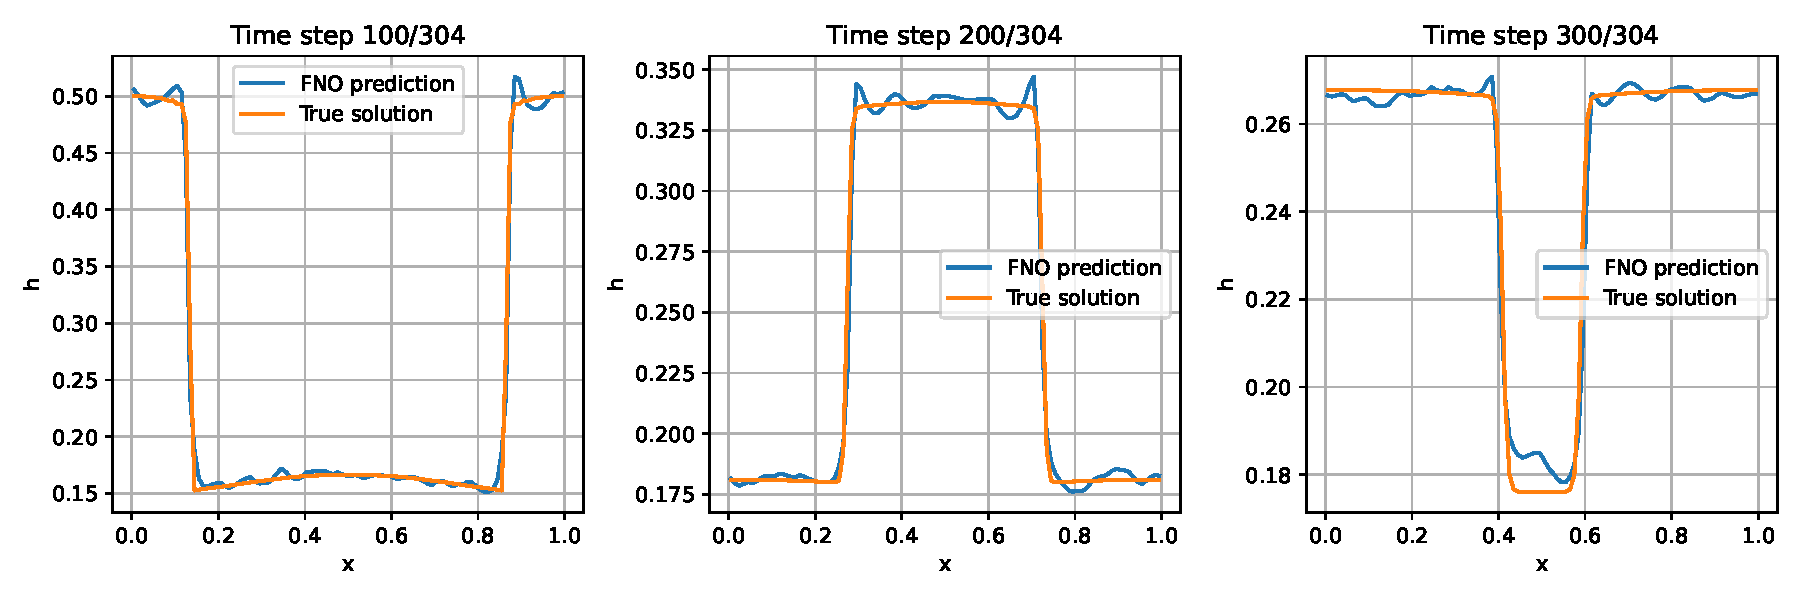
\includegraphics[width=0.9\textwidth]{C:/Users/Matteo/Shallow-Water-Equations/plots/pred_swe_epochs1000_channels64_lr_0.001_timesteps.pdf}
    \caption{FNO predictions timesteps.}\label{fig:FNO_predictions_time_steps}
\end{figure}
\autoref{fig:FNO_predictions_time_steps} demonstrates that the predictions effectively capture the solution's dynamics.
The RMSE for the predictions is shown in \autoref{fig:FNO_rmse}.
\begin{figure}[H]
    \centering
    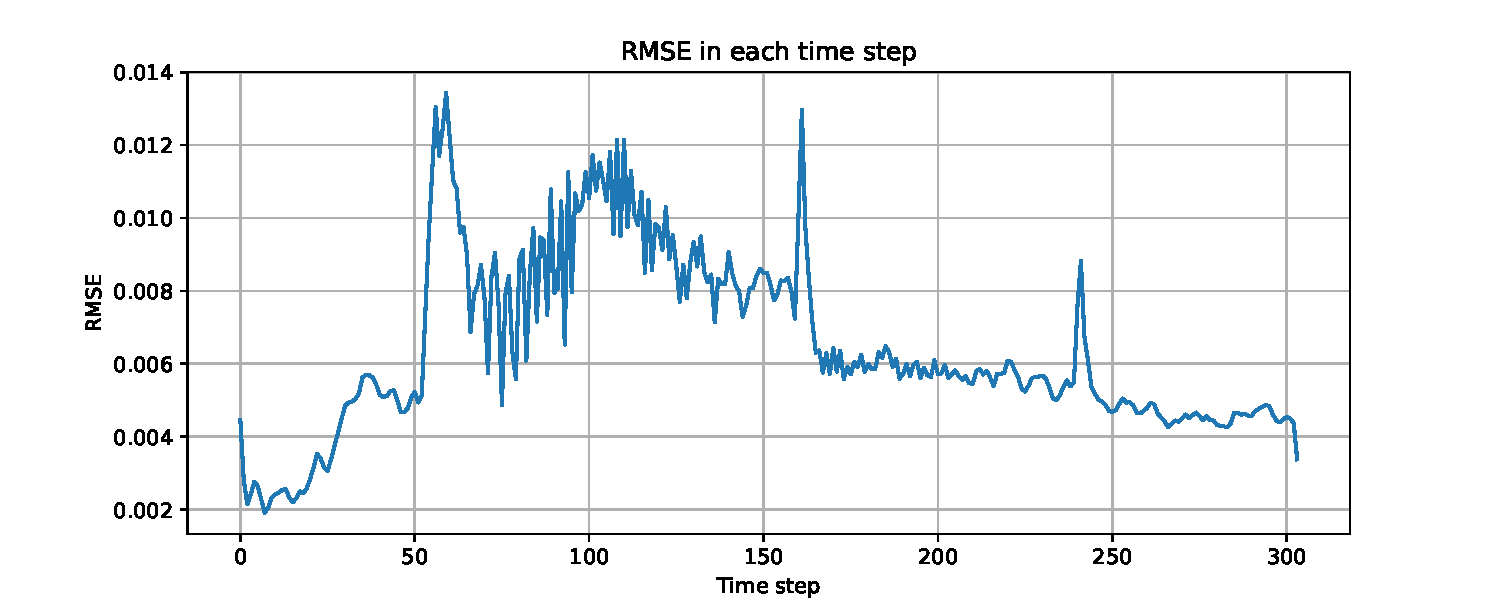
\includegraphics[width=0.7\textwidth]{C:/Users/Matteo/Shallow-Water-Equations/plots/rmse_swe_epochs1000_channels64_lr_0.001.pdf}
    \caption{FNO predictions RMSE.}\label{fig:FNO_rmse}
\end{figure}
From \autoref{fig:FNO_rmse} we see that the RMSE is not increasing for the predictions, which is a good sign.


\subsubsection{FNO Toro test 1}
To test the FNO model on a more challenging problem, we consider the Toro test case 1.
We use the same model as before, but we train it on the data from the Toro test case 1.
Again, we use the first $80\%$ of the data for training and the last $20\%$ for testing.
The results of the model are shown in \autoref{fig:FNO_Toro_test1_predictions_3D} and \autoref{fig:FNO_Toro_test1_predictions}.

\begin{figure}[H]
    \centering
    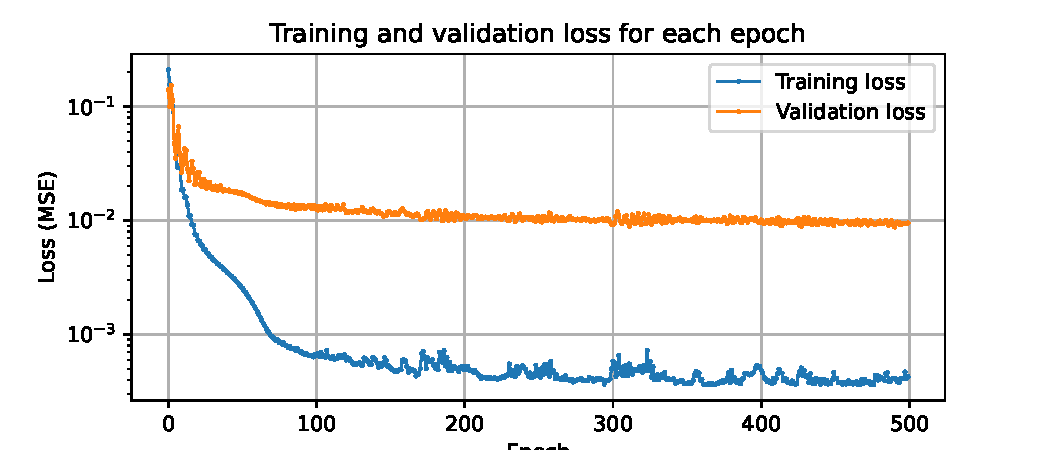
\includegraphics[width=0.7\textwidth]{C:/Users/Matteo/Shallow-Water-Equations/plots/torotest1_loss.pdf}
    \caption{FNO Toro test 1 loss.}\label{fig:FNO_Toro_test1_loss}
\end{figure}

\begin{figure}[H]
    \centering
    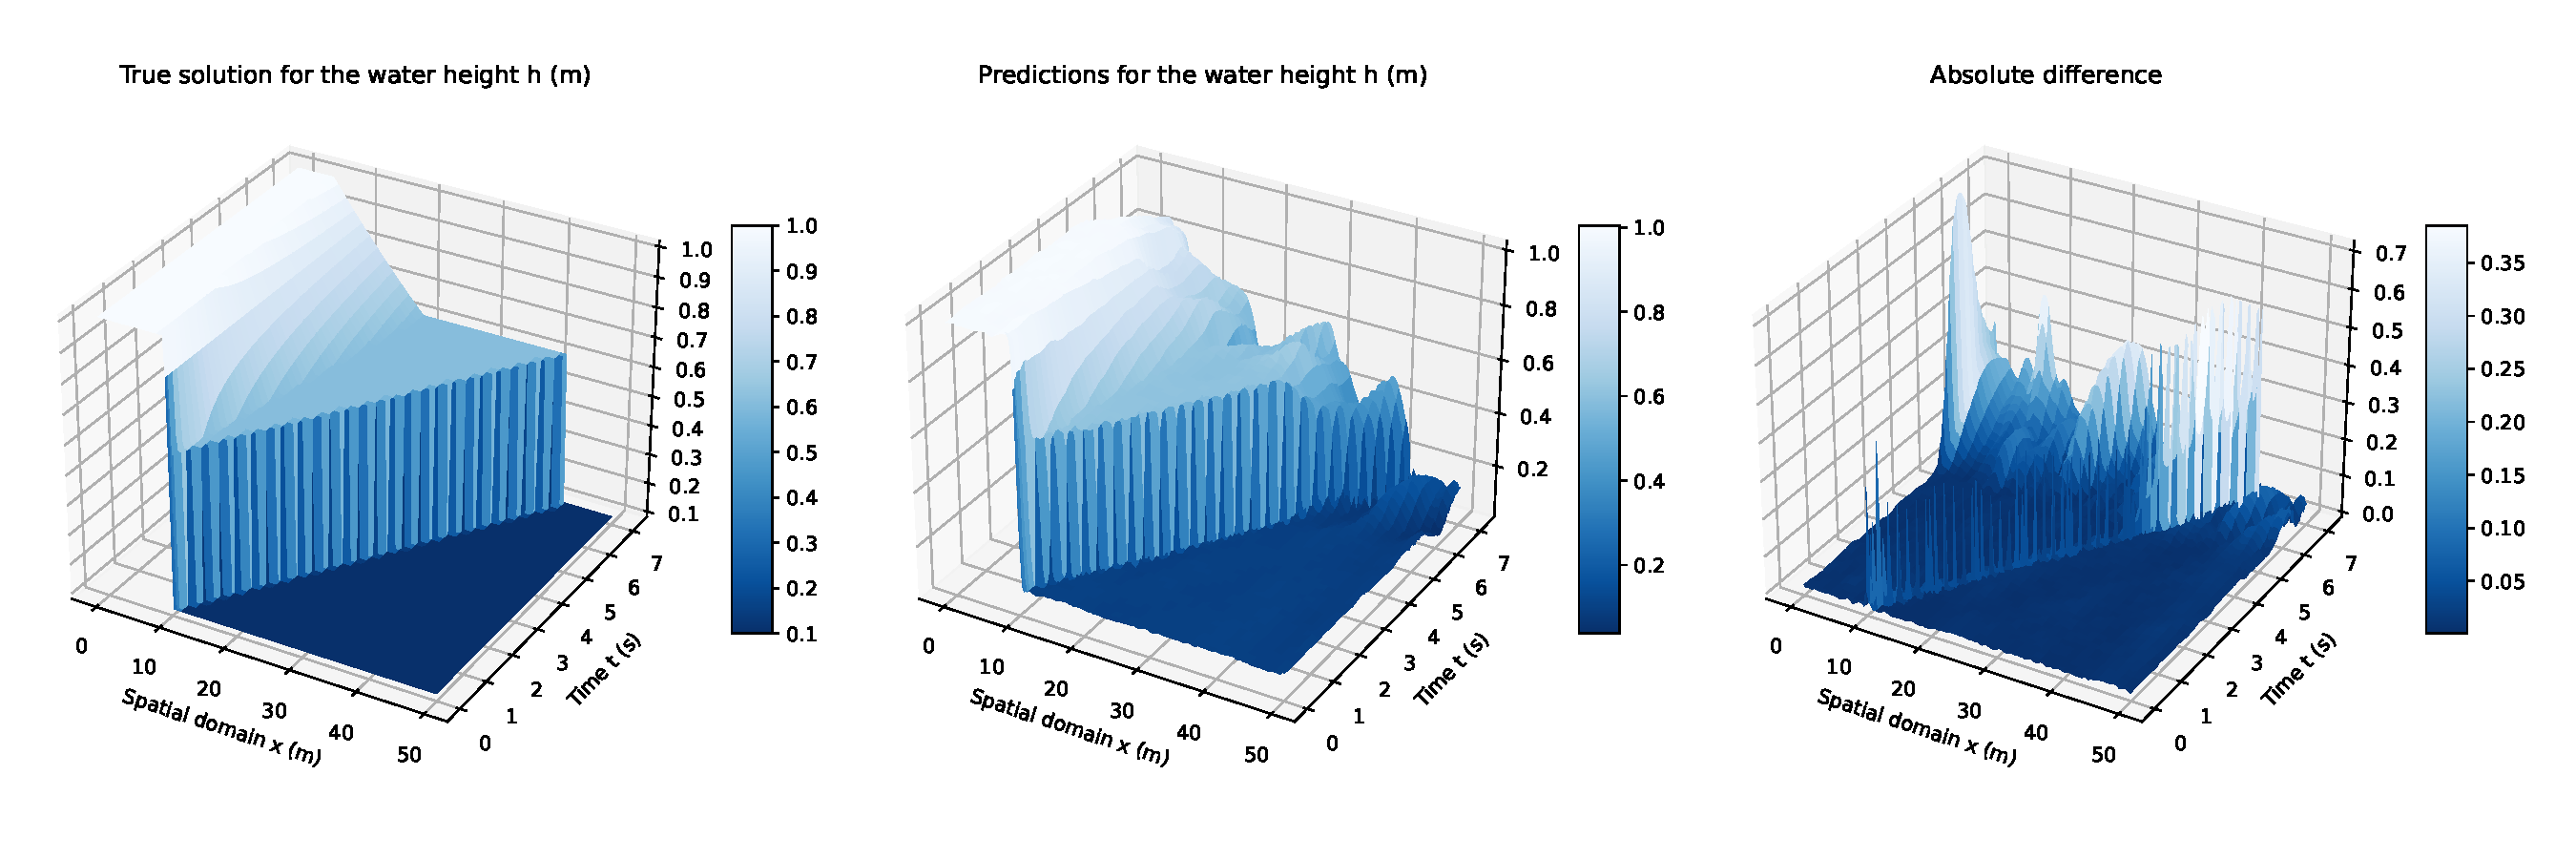
\includegraphics[width=0.9\textwidth]{C:/Users/Matteo/Shallow-Water-Equations/plots/torotest1_predictions_3D.pdf}
    \caption{FNO Toro test 1 predictions in 3d.}\label{fig:FNO_Toro_test1_predictions_3D}
\end{figure}


\begin{figure}[H]
    \centering
    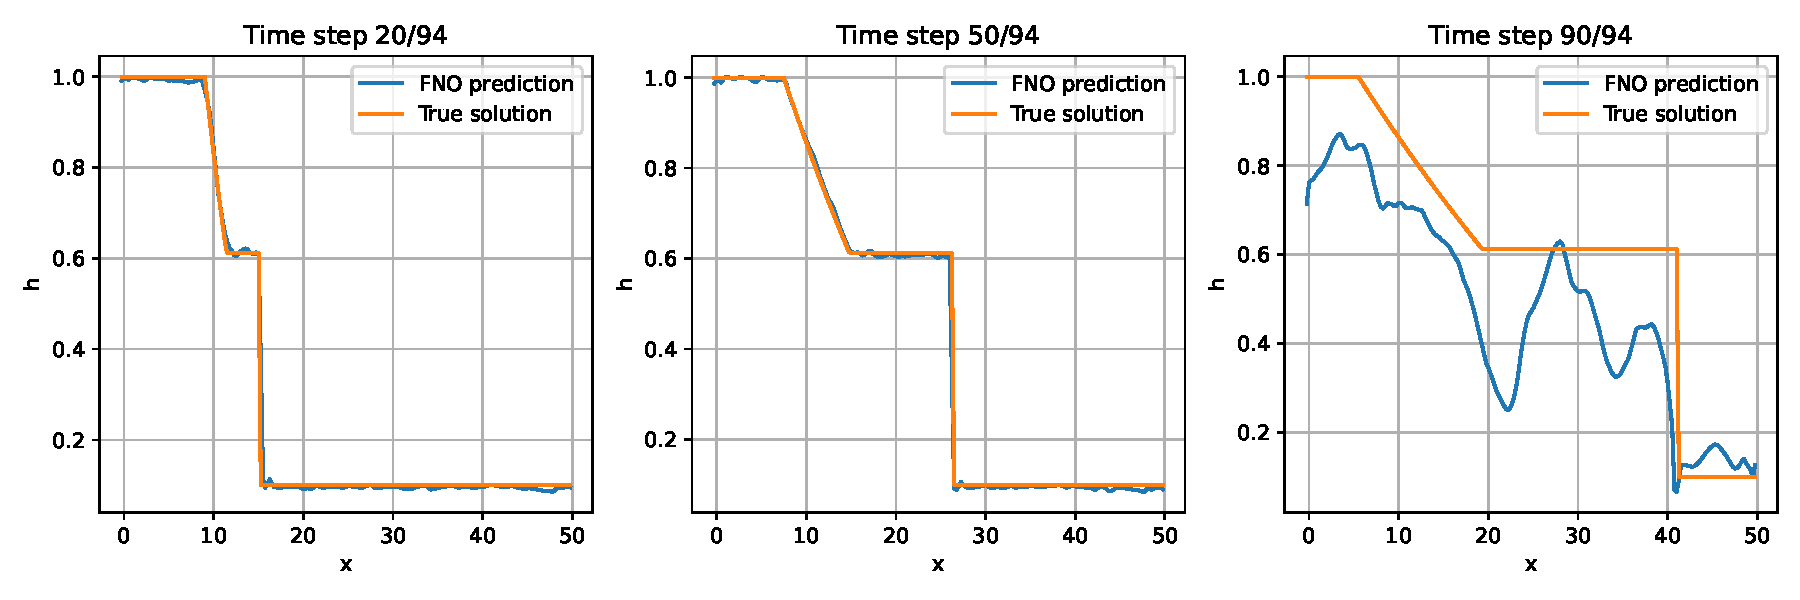
\includegraphics[width=0.9\textwidth]{C:/Users/Matteo/Shallow-Water-Equations/plots/torotest1_predictions_time_steps.pdf}
    \caption{FNO Toro test 1 predictions timesteps.}\label{fig:FNO_Toro_test1_predictions_time_steps}
\end{figure}


\begin{figure}[H]
    \centering
    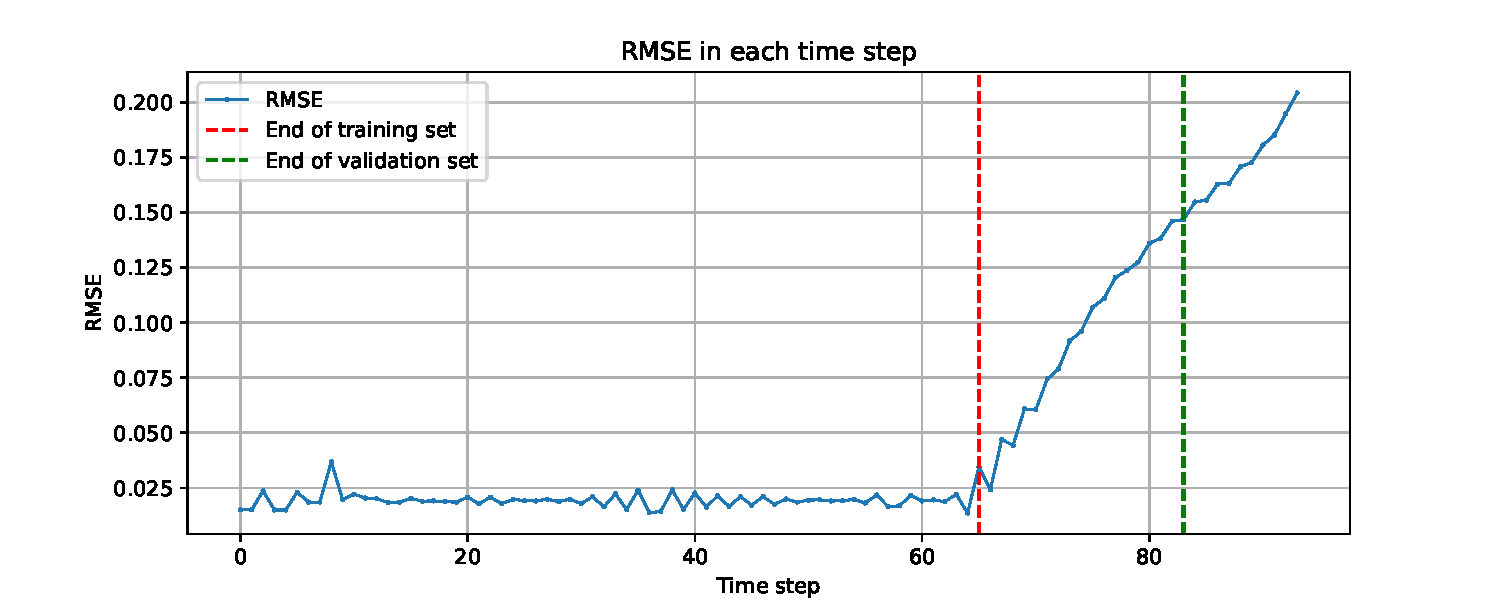
\includegraphics[width=0.7\textwidth]{C:/Users/Matteo/Shallow-Water-Equations/plots/torotest1_RMSE.pdf}
    \caption{FNO Toro test 1 predictions RMSE.}\label{fig:FNO_Toro_test1_rmse}
\end{figure}

\newpage
\subsection{Spherical SWE in 1D}
We also consider the spherical shallow water equations in a 1D setting, focusing on the linearized SWE on a circular domain.
The length of the domain corresponds to the circumreference of the circle, $L = 2\pi$, and is discretized into $N = 500$ points.
The initial conditions is specified as a Gaussian function wrapped around the circle, expressed as:
\begin{align*}
    h(\theta, 0) &= h_0 \exp \left( \frac{-{(\theta-\mu)}^2}{2 \sigma^2} \right) ,\\
\end{align*}
where the parameters are $h_0 = 1, \mu = \frac{\pi}{4}, \sigma = \frac{\pi}{16}$.
The initial conditions can be seen in \autoref{fig:swe_spherical_1d_initial_conditions}.
\begin{figure}[H]
    \centering
    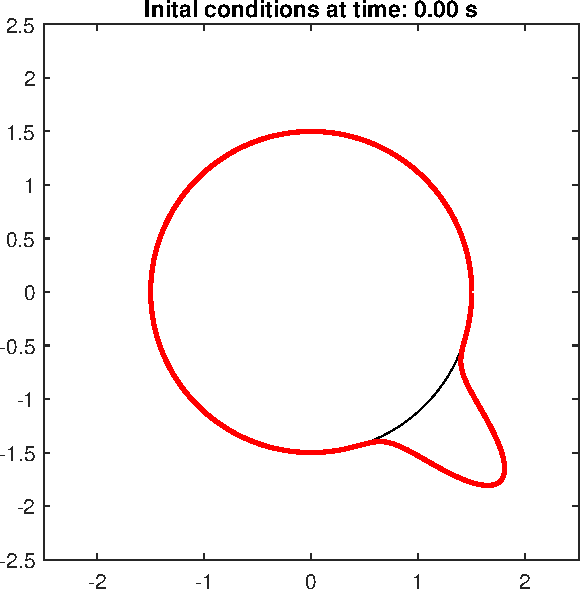
\includegraphics[width=0.4\textwidth]{C:/Users/Matteo/Shallow-Water-Equations/plots/SWE-spherical-1d-initial_conditions.pdf}
    \caption{Initial conditions for the 1D linearized shallow water equations in spherical coordinates.}\label{fig:swe_spherical_1d_initial_conditions}
\end{figure}
The numerical solution in the $\theta,t$ plane is shown in \autoref{fig:Spherical_linear_1D_true_solution}, for $t=0$ to $t=1$.
\begin{figure}[H]
    \centering
    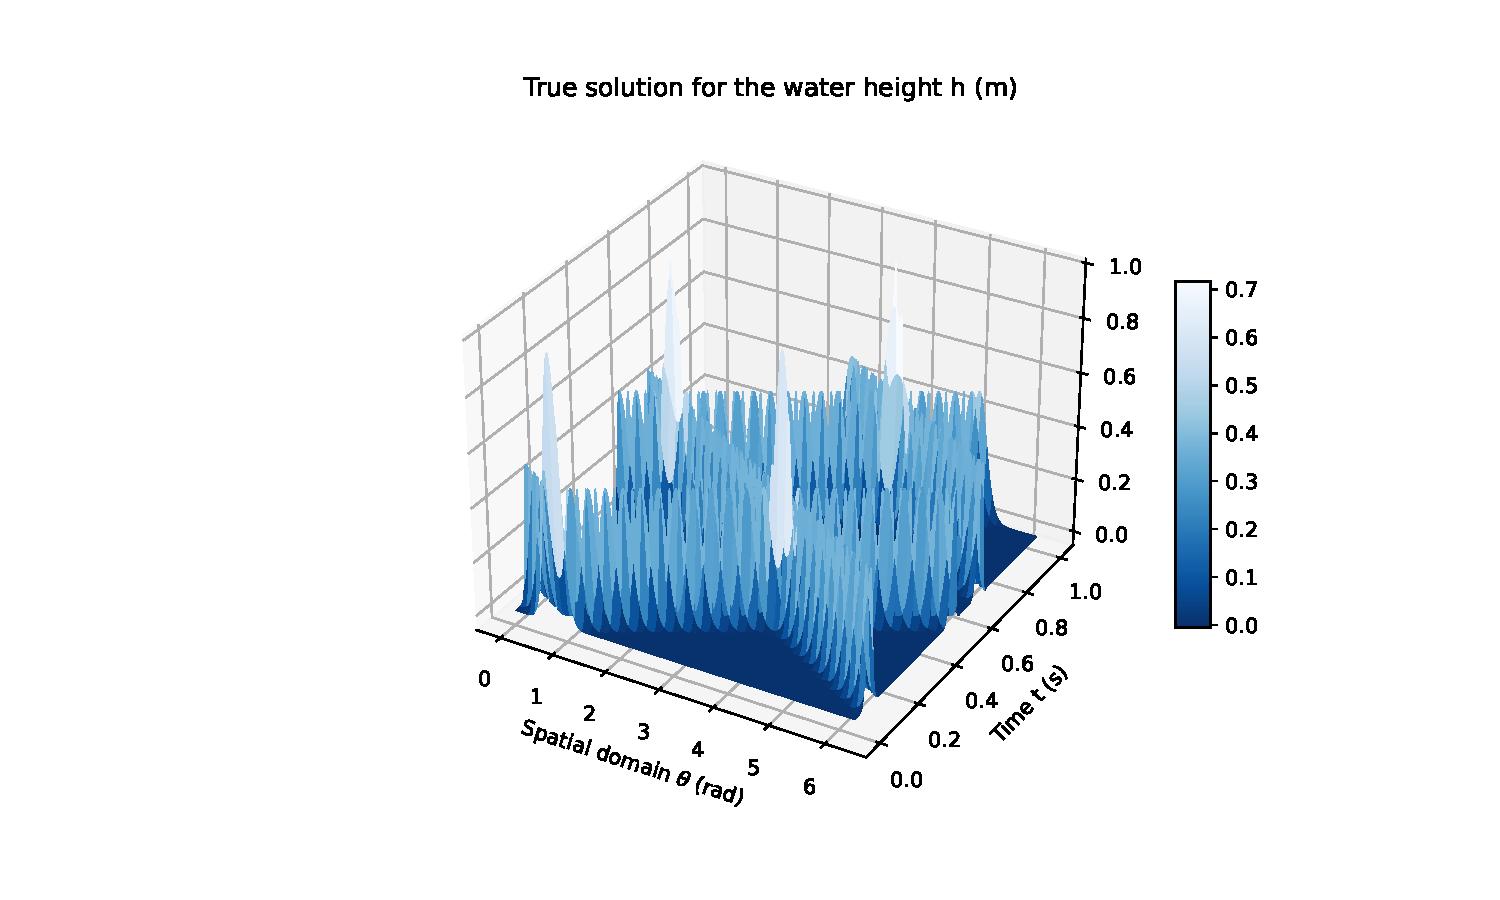
\includegraphics[width=0.8\textwidth]{C:/Users/Matteo/Shallow-Water-Equations/plots/Spherical_linear_1D_true_solution.pdf}
    \caption{Numerical solution of the spherical shallow water equations in 1D in the $\theta,t-$space.}\label{fig:Spherical_linear_1D_true_solution}
\end{figure}
Based on the data generated by the numerical solution (we use time steps of $\Delta t = 0.0025$), we train a FNO model and a Convolutional Neural Network (CNN) model.

\subsubsection{FNO}
The FNO model consists of an input channel, 64 hidden channels and an output channel. We use a Fourier basis with 16 modes and a batch size of 32.
The model is trained using the Adam optimizer with a learning rate of $0.001$, a total of $100$ epochs and the critera is to minimize the mean squared error (MSE).
The model is trained on the data from $t = 0$ to $t = 0.6$, validated on the data from $t = 0.6$ to $t = 0.8$, and tested on the data from $t = 0.8$ to $t = 1.0$.
The training and validation loss is shown in \autoref{fig:Spherical_linear_1D_FNO}.
\begin{figure}[H]
    \centering
    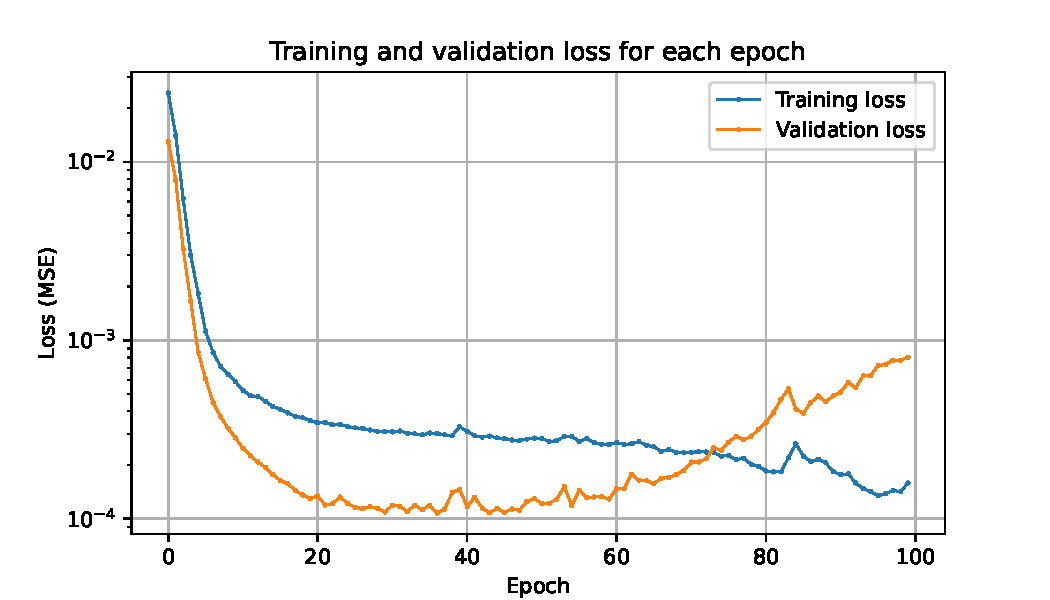
\includegraphics[width=0.7\textwidth]{C:/Users/Matteo/Shallow-Water-Equations/plots/Spherical_linear_1D_FNO.pdf}
    \caption{Training and validation loss for the FNO model for the spherical shallow water equations in 1D.}\label{fig:Spherical_linear_1D_FNO}
\end{figure}
From \autoref{fig:Spherical_linear_1D_FNO} we see that the model is able to learn the dynamics of the solution, but the validation loss is increasing after a certain number of epochs.
The error plots are shown in \autoref{fig:Spherical_linear_1D_FNO_error}.
\begin{figure}[H]
    \centering
    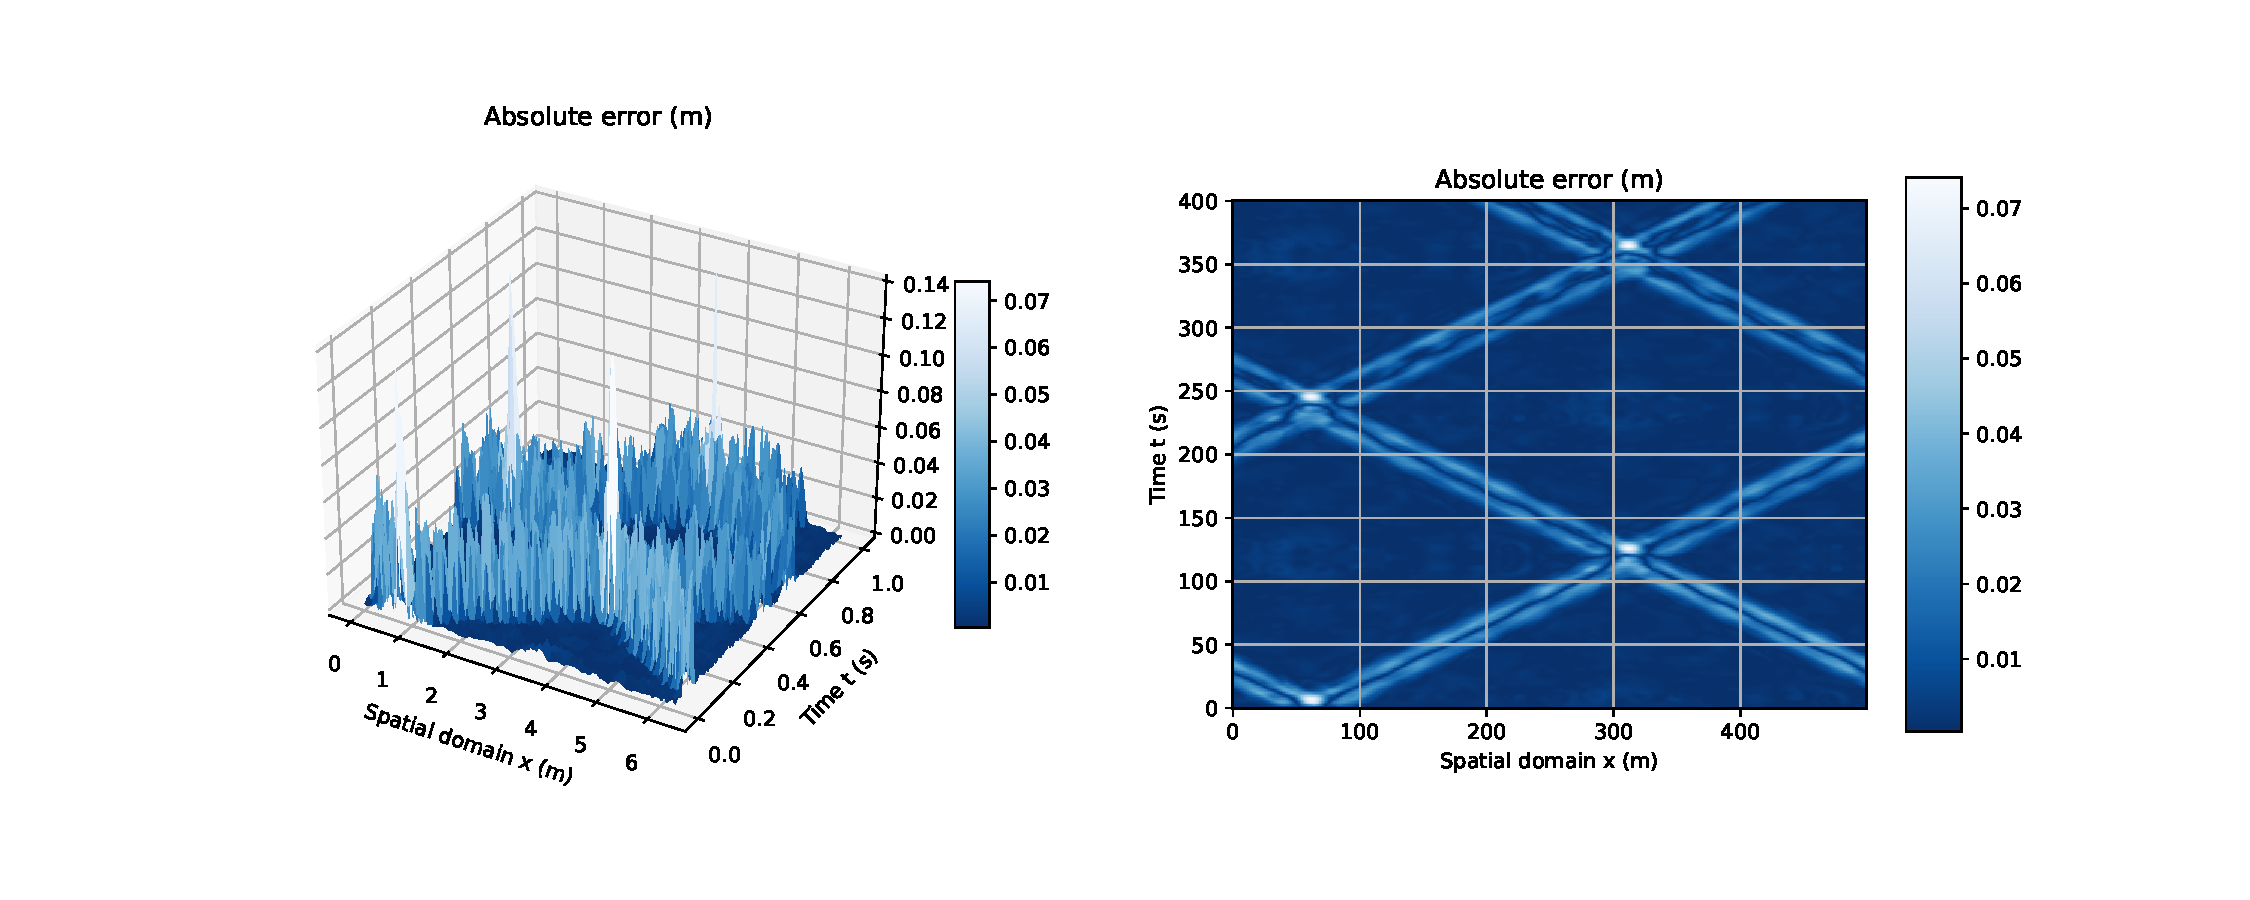
\includegraphics[width=\textwidth]{C:/Users/Matteo/Shallow-Water-Equations/plots/Spherical_linear_1D_FNO_error_sigma=2.pdf}
    \caption{Error plots for the predictions of the 1D linearized spherical SWE.}\label{fig:Spherical_linear_1D_FNO_error}
\end{figure}
From \autoref{fig:Spherical_linear_1D_CNN_error} we see that the model is able to learn the dynamics of the solution.
We also see that the absolute error is biggest at the edges of the solution, which is expected, as the solution tends to be discontinuous.
To get an overview of the performance of the model, we consider the predictions for some given time steps, shown in \autoref{fig:Spherical_linear_1D_FNO_predictions_timesteps}.
\begin{figure}[H]
    \centering
    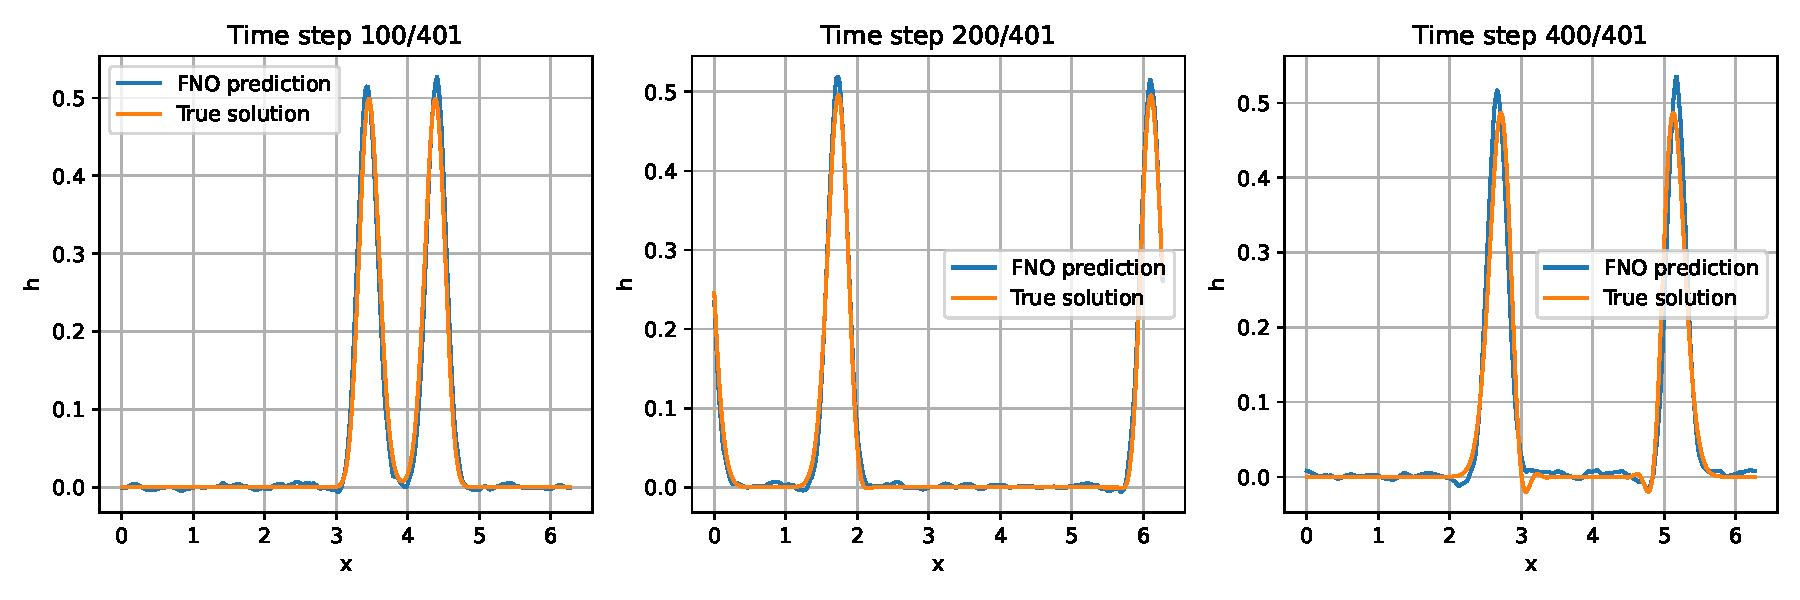
\includegraphics[width=0.9\textwidth]{C:/Users/Matteo/Shallow-Water-Equations/plots/Spherical_linear_1D_FNO_timesteps.pdf}
    \caption{Predictions for the spherical shallow water equations in 1D.}\label{fig:Spherical_linear_1D_FNO_predictions_timesteps}
\end{figure}
From \autoref{fig:Spherical_linear_1D_FNO_predictions_timesteps} we see that the FNO predictions are smooth and rather accurate, but have some small errors in the top of the waves.
Finally we consider the RMSE for the predictions, shown in \autoref{fig:Spherical_linear_1D_FNO_RMSE}.
\begin{figure}[H]
    \centering
    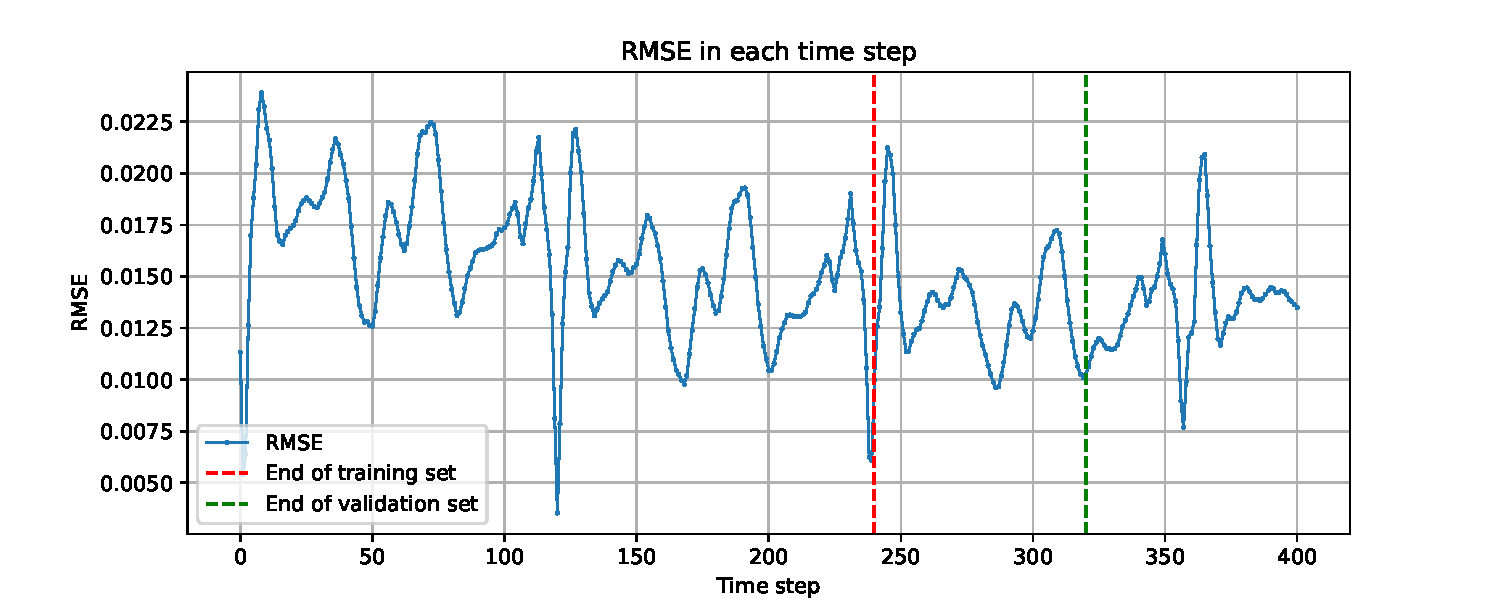
\includegraphics[width=0.7\textwidth]{C:/Users/Matteo/Shallow-Water-Equations/plots/Spherical_linear_1D_FNO_RMSE.pdf}
    \caption{RMSE for the predictions for the spherical shallow water equations in 1D.}\label{fig:Spherical_linear_1D_FNO_RMSE}
\end{figure}
From \autoref{fig:Spherical_linear_1D_FNO_RMSE} we see that the RMSE is not increasing for the predictions, which is a good sign.

\subsubsection{CNN}
We have also trained a CNN model on the data generated by the numerical solution of the SWE in 1D.
Like the FNO model, the CNN model is trained on the data from $t = 0$ to $t = 0.6$, validated on the data from $t = 0.6$ to $t = 0.8$, and tested on the data from $t = 0.8$ to $t = 1.0$.
The training and validation loss is shown in \autoref{fig:Spherical_linear_1D_CNN}.
\begin{figure}[H]
    \centering
    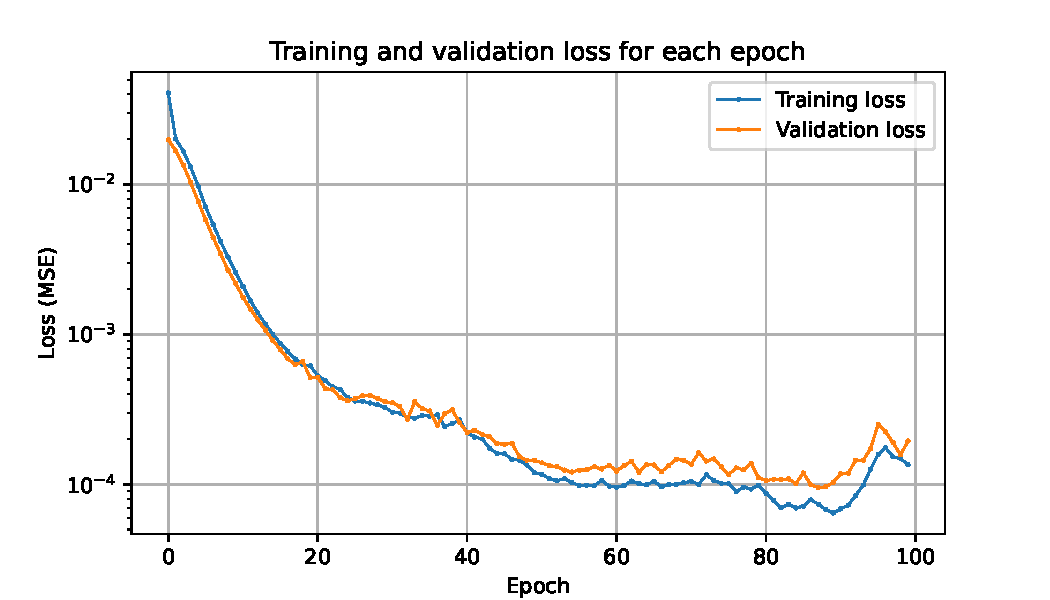
\includegraphics[width=0.7\textwidth]{C:/Users/Matteo/Shallow-Water-Equations/plots/Spherical_linear_1D_CNN.pdf}
    \caption{Training and validation loss for the CNN model for the spherical shallow water equations in 1D.}\label{fig:Spherical_linear_1D_CNN}
\end{figure}

The error plots for the predictions of the CNN model are shown in \autoref{fig:Spherical_linear_1D_CNN_error}.
\begin{figure}[H]
    \centering
    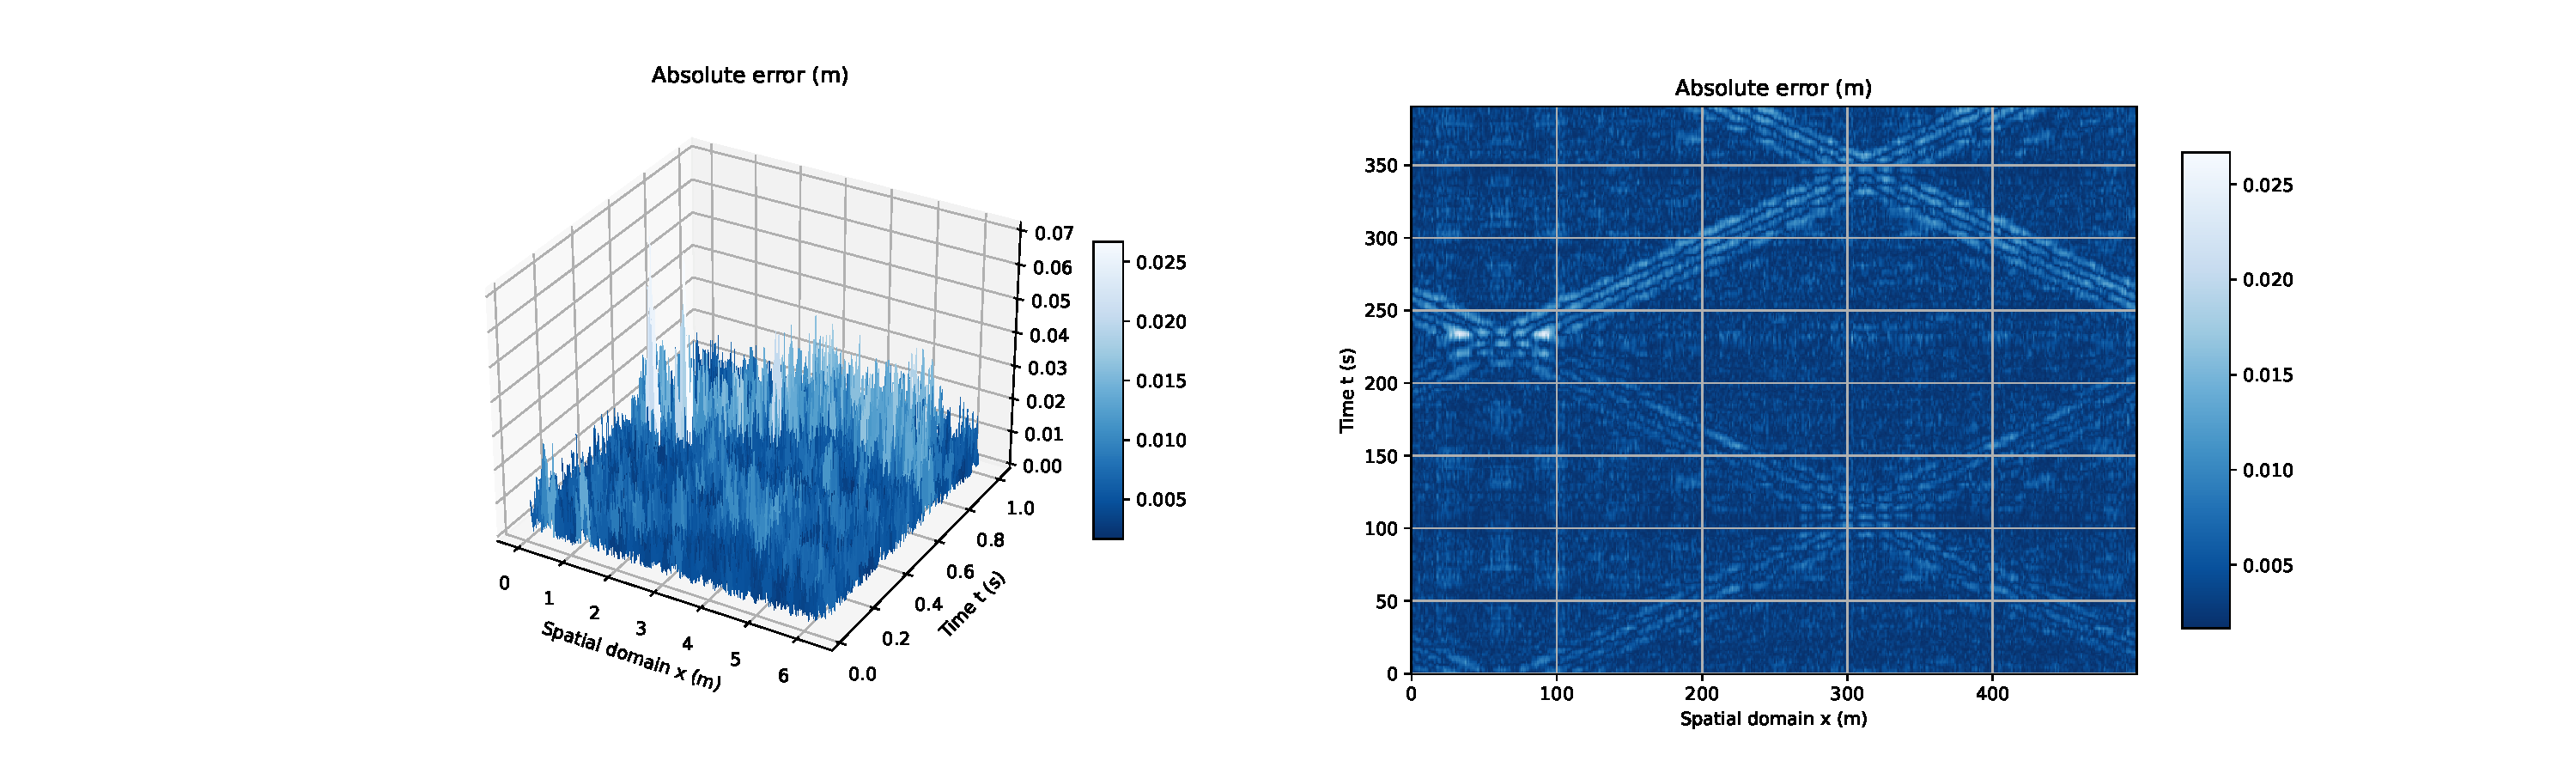
\includegraphics[width=\textwidth]{C:/Users/Matteo/Shallow-Water-Equations/plots/Spherical_linear_1D_CNN_error_sigma=2.pdf}
    \caption{Error plots for the predictions of the CNN model for solving the 1D linearized spherical SWE.}\label{fig:Spherical_linear_1D_CNN_error}
\end{figure}
From \autoref{fig:Spherical_linear_1D_CNN_error} we see that for the CNN model, the errors are more noisy than for the FNO model.
The predictions for some given time steps are shown in \autoref{fig:Spherical_linear_1D_CNN_timesteps}.
\begin{figure}[H]
    \centering
    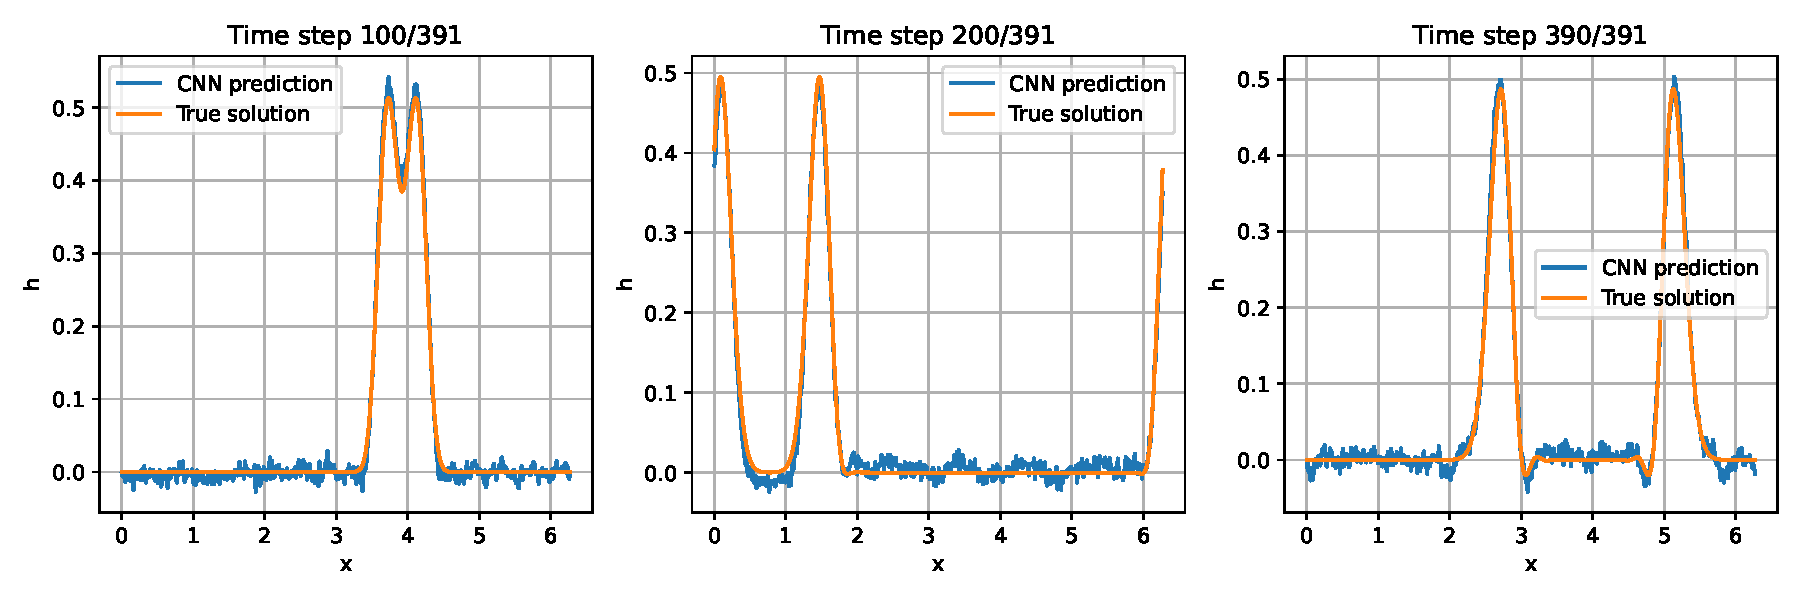
\includegraphics[width=0.9\textwidth]{C:/Users/Matteo/Shallow-Water-Equations/plots/Spherical_linear_1D_CNN_time_steps.pdf}
    \caption{Predictions for the spherical shallow water equations in 1D using the CNN model for some given time steps.}\label{fig:Spherical_linear_1D_CNN_timesteps}
\end{figure}
From \autoref{fig:Spherical_linear_1D_CNN_timesteps}, we also see that the predictions capture the waves, but are more noisy than the FNO predictions.
Finally we consider the RMSE for the predictions, shown in \autoref{fig:Spherical_linear_1D_CNN_RMSE}.
\begin{figure}[H]
    \centering
    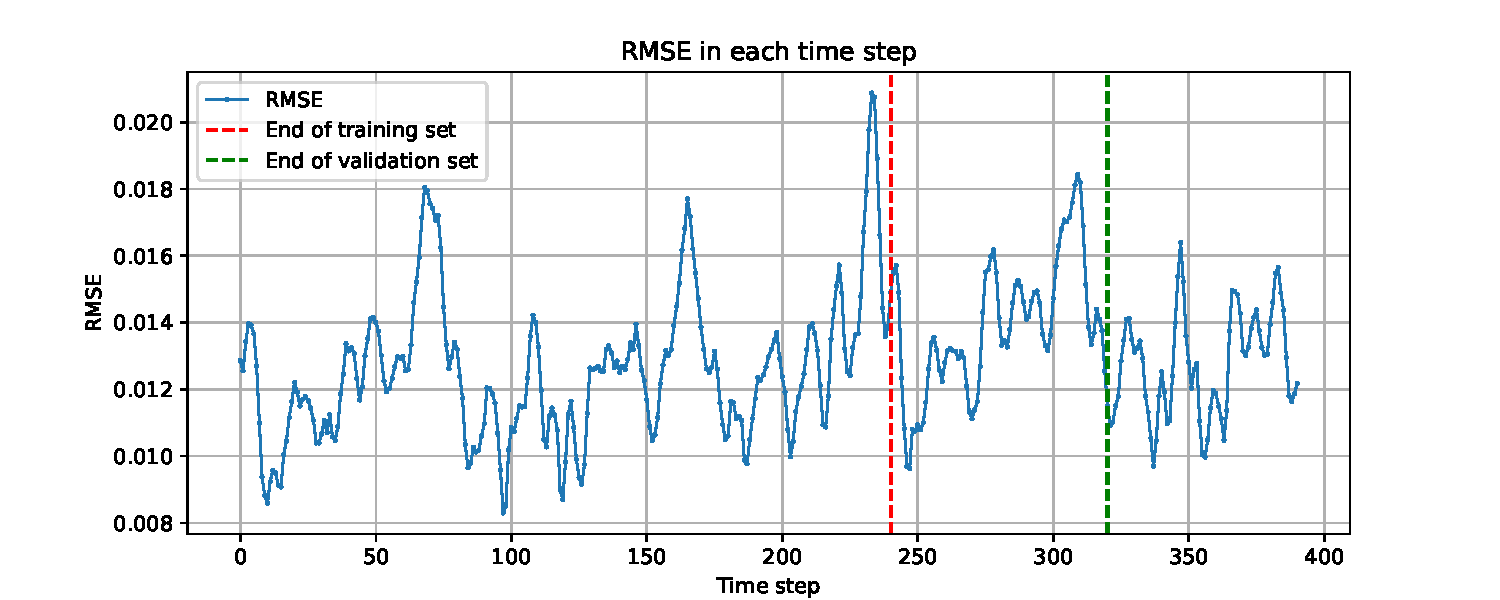
\includegraphics[width=0.7\textwidth]{C:/Users/Matteo/Shallow-Water-Equations/plots/Spherical_linear_1D_CNN_RMSE.pdf}
    \caption{RMSE for the predictions for the spherical shallow water equations in 1D using the CNN model.}\label{fig:Spherical_linear_1D_CNN_RMSE}
\end{figure}

To get an overview of the performance of the different models, we consider the MSE for the predictions for the 1D SWE spherical case.
\begin{table}[H]
    \centering
    \small % Reduce font size
    \begin{tabular}{c|ccc|ccc|ccc}
        \hline
        Model & \multicolumn{3}{c|}{$\sigma = \pi/8$} & \multicolumn{3}{c|}{$\sigma = \pi/16$} & \multicolumn{3}{c}{$\sigma = \pi/32$} \\
        \cline{2-10}
        & MSE & MAE & Time (s) & MSE & MAE & Time (s) & MSE & MAE & Time (s) \\
        \hline
        CNN & 6.72e-05 & 6.48e-03 & 93.71 & 1.35e-04 & 8.40e-03 & 98.77 & 3.06e-04 & 1.25e-02 & 96.53 \\ 
        \hline
        FNO & 2.25e-04 & 9.78e-03 & 133.87 & 1.47e-04 & 7.12e-03 & 109.65 & 4.44e-04 & 1.07e-02 & 108.69 \\ 
        \hline
    \end{tabular}
    \caption{Test loss in terms of MSE and MAE, and time for training the models for the 1D spherical SWE.}\label{tab:results_spherical_1D_comparison}
\end{table}
From \autoref{tab:results_spherical_1D_comparison} we see that the CNN model is slightly faster and better than the FNO model for $\sigma = \pi/8$ and $\sigma = \pi/16$, but for $\sigma = \pi/32$, the performance of the CNN model is decreasing.
Probably due to the fact that the smaller the $\sigma$, the more discontinuous the solution is, and the FNO model is better at capturing the discontinuities.
We see that the MAE in general is higher than the MSE, and is also increasing for smaller $\sigma$.
Additionally, we observe that the MAE is higher, as it places more weight on small errors compared to the MSE.
And in the CNN case we see a lot of small errors/noise, which is why the MAE is higher than the MSE.



\newpage
\subsection{Comparison}
To get an overview of the performance of the different models, we consider the RMSE for the predictions for the smooth case.
We consider the MSE for the whole data set, and the time for training the model.
\begin{table}[H]
    \centering
    \begin{tabular}{c|c|c}
        \hline
        \text{Model} & \text{MSE} & \text{Time}\\
        \hline\hline
        \text{RNN} & $8.71 \cdot 10^{-4}$ &  464.13 s \\ 
        \hline
        \text{FNO} & $3.70 \cdot 10^{-6}$ & 383.60 s  \\
        \hline
    \end{tabular}
    \caption{MSE and time for training the models for the smooth case.}\label{tab:RMSE_smooth}
\end{table}

\begin{table}[H]
    \centering
    \begin{tabular}{c|c|c}
        \hline
        \text{Model} & \text{MSE} & \text{Eval time} \\
        \hline\hline
        \text{RNN} &  &  \\ 
        \hline
        \text{FNO} &  &  \\
        \hline
    \end{tabular}
    \caption{RMSE and evalutation time for the predictions for the Toro test case 1.}\label{tab:torotest1}
\end{table}









